\documentclass[10pt]{beamer}
\usetheme{Madrid}
\usecolortheme{beaver}
\usepackage{tikz}
\usetikzlibrary{automata, positioning, arrows}

\title[Sequence Detector]
{Sequence Detector}
\subtitle{DCS Final Presentation}
\institute{DTU}
\author{Jatin Pandey \& kumood}
\logo{
  \includegraphics[height=1cm]{./src/logo.png}
}
\begin{document}
  \frame {
      \titlepage
    }
  \frame {
      \frametitle{What is a Sequence Detector?}
      A sequence detector accepts as input a string of bits: either 0 or 1.   Its output goes to 1 when a target sequence has been detected.
    }
  \frame{
      \frametitle{Types of Sequence Detector}
      There are two basic types of Sequence Detector
      \begin{itemize}
        \item Overlap
        \item Non-Overlap
      \end{itemize}
    }
  \frame{
        \frametitle{Simple Finite State Machine}

        \begin{figure}[ht] % ’ht’ tells LaTeX to place the figure ’here’ or at the top of the page
          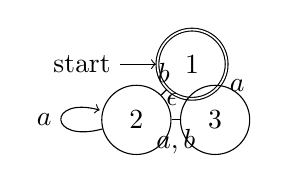
\begin{tikzpicture}
            % tikz code goes here
            \node[state, initial, accepting] (1) {$1$};
            \node[state, below left of=1] (2) {$2$};
            \node[state, right of=2] (3) {$3$};
            \draw (1) edge[above] node{$b$} (2)
            (1) edge[below, bend right, left=0.3] node{$\epsilon$} (3)
            (2) edge[loop left] node{$a$} (2)
            (2) edge[below] node{$a, b$} (3)
            (3) edge[above, bend right, right=0.3] node{$a$} (1);
          \end{tikzpicture}
          \caption{Caption of the FSM}
          \label{fig:my_label}
        \end{figure}
    }
\end{document}
